\glsreset{CA-ML}
\glsreset{ILS}
\glsreset{MSC}
\glsreset{GTEE}
\glsreset{AD}
\glsreset{ML}
\glsreset{RF}
\glsreset{MSA}
\glsreset{FP}
\glsreset{FN}
\section{Introduction}
\label{sec:include-intro}
\glsreset{genefiltering}
Of the dominant approaches for estimating \glspl{speciestree} in the presence of \gls{ILS}, \glspl{genetreesummarymethod} are growing in popularity, as many are provably \gls{statisticallyconsistent} under the \gls{MSC} model as well as computationally efficient compared to \gls{CA-ML}.
However, \gls{GTEE} and \gls{missingdata} can negatively impact summary methods, and some researchers have concerns about their validity under biologically realistic conditions \cite{gatesy2014phylo, springer2016gene}.
As a result, \gls{genefiltering} based on missing data or proxies for GTEE is an increasingly explored aspect of experimental design.
Filtering data, both \glspl{site} and \glspl{gene}, has a long history in phylogenetics; see \cite{streicher2016how, wiens2011missing, chen2015selecting} for an entry into this literature. 
Many of these prior studies (e.g., \cite{wiens2011missing, cho2011can, salichos2013inferring, salichos2014novel, betancur2014conserved, jiang2014should, dornburg2014phylogenetic, streicher2016phylogenomic, dornburg2017new}) have focused on CA-ML and/or datasets simulated without \gls{genetreeheterogeneity}, so their results are not directly applicable to understanding the effect of gene filtering on \glspl{coalescentmethod}.

Some recent studies examine this issue on biological datasets (e.g., \cite{liu2015estimating, chen2015selecting, xi2015genes, hosner2016empirical, huang2016unforeseen, meiklejohn2016analysis, simmons2016effects, streicher2016how, longo2017phylogenomic, blom2017accounting}).
Because accuracy cannot be evaluated on biological datasets, different proxies for accuracy were reported, including
\begin{itemize} 
	\item the mean \gls{bootstrapsupport} of the estimated species tree, 
	\item the bootstrap support of well-established clades in the estimated species tree, 
	\item the similarity of species trees estimated from the same dataset using different methods, and
	\item the ``stability'' of the estimated species tree (comparing the species trees estimated using the same method but given subsets of the genes). 
\end{itemize}
These studies came to contradictory conclusions: some found filtering to be beneficial, while others found filtering to be detrimental.
\Glspl{simulationstudy} have shown that species tree estimation methods can produce highly supported \gls{FP} branches under some model conditions; see \cite{kubatko2007inconsistency} for an example with CA-ML when ILS is high and \cite{bayzid2015weighted} for an example with summary methods when GTEE is high.
Therefore, high bootstrap support or similarity to another estimated species trees may not be reliable indicators of species tree accuracy.

To the best of our knowledge, only three prior simulation studies \cite{liu2015estimating, huang2016unforeseen, lanier2014how} have directly or indirectly examined the impact of gene filtering on coalescent methods. 
First, Lanier {\em et al.} \cite{lanier2014how} added genes with lower variation when using \gls{STEM} on datasets with eight species. 
Second, Liu {\em et al.} \cite{liu2015estimating} added genes with lower bootstrap support values when using \gls{MP-EST} on datasets with six species. 
Third, Huang and Knowles \cite{huang2016unforeseen} filtered genes with missing data when using the \textit{\gls{shallowestdivergence}} method (a coalescent method that takes site patterns as input) \cite{takahata1989gene-msd} on datasets with eight species.
While none of these studies found filtering to be beneficial, many new coalescent methods are now in active use, and the effect of gene filtering likely depends on the method itself as well as on the model condition (e.g., number of species, number of genes, level of ILS, amount of phylogenetic signal across individual genes, etc.) \cite{liu2009estimating-star}.
Hence, a thorough evaluation of gene filtering is needed, especially to examine its effect on some of the current leading species tree estimation methods.

We present the results of a simulation study examining the impact of ISL, phylogenetic signal (across individual genes), missing data, and gene filtering strategies on five species tree estimation methods: \gls{ASTRAL}-II,  \gls{ASTRID}, MP-EST, \gls{SVDquartets}, and CA-ML using \gls{RAxML}. 
In this study, summary methods (ASTRAL-II, ASTRID, and MP-EST) were more accurate than CA-ML, provided that ILS was sufficiently high and GTEE was sufficiently low. 
When GTEE was sufficiently high, SVDquartets was more accurate than the summary methods, but otherwise it was one of the least accurate. 
CA-ML was competitive with (and often outperformed) the other methods under many conditions, including when ILS and GTEE were both extremely high. 
In general, the relative performance of methods was unaffected by gene filtering based on either GTEE or missing data. 
SVDquartets and CA-ML did not benefit from either type of filtering, and filtering based on missing data generally reduced accuracy. 
Filtering genes based on GTEE improved the accuracy of summary methods when the level of ILS was sufficiently low but otherwise reduced accuracy. 
Exceptions to this trend occurred when the level of GTEE was extremely high, in which case filtering based on GTEE improved summary methods. 
Importantly, these exceptions were for model conditions with only a few replicates: two replicates with low/moderate ILS, five replicates with high ILS, and 17 replicates with very high ILS.

\section{Performance Study}
\label{sec:include-study}
Our study evaluated three summary methods (ASTRAL-II,   ASTRID, and MP-EST), one \gls{site-basedmethod} (SVDquartets), and CA-ML (using RAxML) on a collection of datasets originally simulated by Mirarab {\em et al.} \cite{mirarab2015astral2}. 
We modified these simulated datasets to produce a range of model conditions from relatively easy (e.g., low/moderate ILS, moderate GTEE, and no missing data) to very challenging (e.g., high ILS, high GTEE, and missing data). 
To explore the impact of gene filtering, genes were removed from datasets prior to species tree estimation based on either GTEE or missing data. 
Methods were evaluated based on the species tree estimation error, as measured by the \gls{RFerrorrate} (Equation~\ref{eq:rf-error}).
All software commands are provided in the Supplementary Materials.

\subsection{Simulated Datasets}
In this section, we provide a brief overview of the simulation protocol used by Mirarab {\em et al.} \cite{mirarab2015astral2} and describe our modifications to their datasets.

\paragraph{Species trees and gene trees:} 
Mirarab {\em et al.} \cite{mirarab2015astral2} used \gls{SimPhy} \cite{mallo2016simphy} to simulate a collection of 200-species, $1\,000$-gene datasets under the MSC model with six different model conditions: three levels of ILS with either deep or recent speciation.
Because MP-EST is computationally intensive on datasets with 50 species \cite{bayzid2014disk, mirarab2015astral2}, we restricted datasets to 26 species (outgroup species and 25 randomly selected species) and used only 20 (out of the original 50) replicates.

After restricting datasets to 26 species, we computed several statistics that reflect the level of ILS: \gls{AD} between the model species tree and the gene trees, the number of model species trees in the \gls{anomalyzone} (based an empirical estimate), and the number of distinct gene tree \glspl{topology}.
The mean AD ($\pm$ standard deviation) across replicate datasets was $12 \pm 2$\% for the ``low/moderate'' ILS  condition, $41\pm6$\% for the ``high'' ILS condition, and $75\pm1$\% for the  ``very high'' ILS condition.
Under the low/moderate ILS condition, 20\% of the replicate datasets with recent speciation and 60\% of the replicate datasets with deep speciation were in the anomaly zone; the number of distinct gene tree topologies was also high: there were 344--442 different topologies (out of $1\,000$) for replicates with recent speciation events and 509--824 different topologies (out of $1\,000$) for replicates with deep speciation events.
Hence, while AD was only 12\%, gene tree heterogeneity in this ``low/moderate'' ILS condition was still substantial; this condition is representative of species trees with a mixture of short and long edges (in \glspl{coalescentunit}), perhaps with a small \gls{rapidradiation} creating the anomaly zone.
In the other model conditions (high and extremely high ILS), 100\% of the replicates were in the anomaly zone, and each replicate had 999 or $1\,000$ distinct gene tree topologies.
These high and extremely high levels of ILS are representative of a single clade that has undergone a rapid radiation, so nearly every edge is short.
In summary, all model conditions explored have a high incidence of species trees in the anomaly zone but differ with respect to the fraction of branches in the species tree that are short enough for coalescence to be likely.

\paragraph{DNA (gene) sequence data:} Mirarab {\em et al.} \cite{mirarab2015astral2} used \gls{INDELible} \cite{fletcher2009indelible} to simulate DNA sequence data under the \gls{GTR+GAMMA} model with variable lengths (300--1500 sites) from each model gene tree (with branch lengths deviating from a \gls{strictmolecularclock}).
We modified the gene \glspl{MSA} to have shorter lengths (truncating them to the first 100 sites) to produce conditions with fewer \gls{parsimony-informative} sites and thus higher GTEE. 
Such conditions may be characteristic of datasets where genes are shortened to avoid \gls{recombination} (e.g., \cite{hobolth2011incomplete}) or where gene trees have low bootstrap support (e.g., \cite{jarvis2014whole, wickett2014phylo, hosner2016empirical, blom2017accounting}). 

\paragraph{Missing data:} We modified the gene MSAs (by deleting sequences) to produce conditions with missing data biased towards a random subset of genes.
The final datasets had 250 genes missing between 13--19 sequences (i.e., 50--73\%), 250 genes missing between 7--12 sequences (i.e., 27--46\%), 250 genes missing between three to six sequences (i.e., 12--23\%), 150 genes missing two sequences (i.e., 8\%), 50 genes missing one sequence (i.e., 4\%), and 50 genes missing zero sequences (Supplementary Table S2). 
The total amount of missing data was approximately 30\% for all datasets.
Note that our protocol for producing datasets with missing data was based on an empirical dataset published by Hosner {\em et al.} \cite{hosner2016empirical}, which shows that the percentage of missing data varies across genes but is uncorrelated with evolutionary rate (Supplementary Table S1 and Supplementary Figure S1).

\paragraph{Estimated gene trees:}
We estimated \gls{ML} gene trees under the GTR+GAMMA model using RAxML version 8.2.8 with a single tree search. 
For each replicate dataset, mean GTEE was computed as the normalized \gls{RF} distance between a true gene tree and its respective estimated gene tree, averaged across all $1\,000$ genes. 
Replicates were partitioned based on their mean GTEE as follows. 
Replicates with the full length sequences (300--1500 sites) were partitioned into {\em low/moderate} GTEE (i.e., mean GTEE between 0--20\%) and {\em moderate/high} GTEE (i.e., mean GTEE between 20--50\%). 
The mean GTEE averaged ($\pm$ standard deviation) across all replicates with the full length sequences was $16 \pm 2\%$ and $35 \pm 8\%$ for {\em low/moderate} and {\em moderate/high} GTEE, respectively (Supplementary Tables S3--S4). 
Replicates with the truncated sequences (100 sites) had higher GTEE and were partitioned into {\em very high} GTEE (i.e., mean GTEE within 50--80\%) and {\em extremely high} GTEE (i.e., mean GTEE within 80--100\%). 
The mean GTEE averaged ($\pm$ standard deviation) across datasets with truncated sequences was $69 \pm 8\%$ and $86 \pm 5\%$ for {\em very high} and {\em extremely high} GTEE, respectively (Supplementary Tables S5--S6).

\subsection{Gene Filtering Experiments}
We evaluated the impact of gene filtering by removing 0\%, 25\%, 50\%, 75\%, 90\%, and 95\% of the genes, producing a collection of datasets that varied in the number of genes retained for species tree estimation. 
To filter genes by GTEE, gene trees were sorted from lowest to highest GTEE, and then the top 0\%, 25\%, 50\%, 75\%, 90\%, and 95\% of genes were removed prior to species tree estimation. 
To filter genes by missing data, gene trees were sorted based on the amount of missing data (i.e., the fraction of species deleted from the gene sequence alignment), and then genes missing greater than or equal to 50\%, 25\%, 10\%, 5\%, or 1\% of the species were removed prior to species tree estimation. 
These thresholds for GTEE and missing data resulted in the same number of genes being removed, making the two filtering experiments comparable.

\subsection{Species Tree Estimation}
We evaluated five species tree estimation methods: three summary methods (ASTRAL-II version 4.10.5, ASTRID version 1.1, and MP-EST version 1.5), a site-based method (SVDquartets as implemented in \gls{PAUP*} version 4a150), and CA-ML (using RAxML version 8.2.8 under the GTR+GAMMA).
Of these methods, only ASTRAL-II returns species trees with branch lengths annotated by statistical support; its technique for computing support values has been shown to be a better predictor of topological accuracy than \textit{\gls{MLBS}} \cite{sayyari2016fast}.
ASTRAL-II and ASTRID were given \gls{unrooted} ML gene trees as input.
MP-EST was given ML gene trees \gls{rooted} at the outgroup species (when available) or at the midpoint of the longest leaf-to-leaf path.
The best pseudo-likelihood scoring species tree was taken from ten independent runs of MP-EST.

\section{Results}
\label{sec:include-results}
We now present the results of four experiments. 
The first and second evaluate the impact of ILS and phylogenetic signal (across individual genes) on five species tree estimation methods with and without missing data, respectively.
The third and fourth evaluate the impact of gene filtering based on GTEE and missing data, respectively. 

\subsection{Impact of Incomplete Lineage Sorting and Phylogenetic Signal} 
For all methods, mean species tree error increased as ILS and/or phylogenetic signal increased, but the relative performance between methods depended on both ILS and phylogentic signal (Figure~\ref{fig:include-1}). 
Phylogenetic signal is reported as mean GTEE, so low phylogenetic signal (per gene) corresponds to high mean GTEE and high phylogenetic signal (per gene) corresponds to low mean GTEE.

For low/moderate ILS (12\% AD), CA-ML was the most accurate method for all levels of GTEE (Figure~\ref{fig:include-1}a). 
When mean GTEE was less than 50\%, all five methods had good accuracy (mean species tree error below 7\%). 
When mean GTEE was between 80--85\%, the differences between methods were noteworthy; the mean species tree error was 5\% for CA-ML, ranged for summary methods (from 16\% for ASTRAL-II to 19\% for MP-EST), and was 20\% for SVDquartets. 
Notably, this model condition had only five replicates.

For high ILS (41\% AD), the relative performance between methods changed dramatically with GTEE (Figure~\ref{fig:include-1}b). 
The three summary methods outperformed SVDquartets and CA-ML when GTEE was low to moderate (i.e., mean GTEE $<50\%$), but SVDquartets and CA-ML outperformed all summary methods when GTEE was extremely high. 
CA-ML produced more accurate species trees than SVDquartets except for the highest GTEE condition (a model condition with only four replicates), where both methods had similar accuracy.

For very high ILS (75\% AD), results were similar but more pronounced than those observed for the high ILS condition (Figure~\ref{fig:include-1}c). For lower levels of GTEE, CA-ML and SVDquartets were distinctly worse than the summary methods but still provided reasonable accuracy. All methods decreased in accuracy as the level of GTEE increased, but the accuracy of SVDquartets and CA-ML decreased more gradually than all summary methods. When mean GTEE was at least 90\% (a model condition with only four replicates), the differences between methods were dramatic: the mean species tree error for all summary methods was greater than 90\%, while the mean species tree error for CA-ML and SVDquartets was much lower at 30\% and 37\%, respectively.

In summary, both ILS and GTEE had strong effects on the absolute and relative performance of methods. 
All summary methods typically outperformed or else matched the accuracy of CA-ML when GTEE was sufficiently low, but they were less accurate when GTEE was high. 
Although SVDquartets was dramatically more accurate than all summary methods under the most difficult conditions (with very high GTEE and very high ILS), SVDquartets was nearly always outperformed by CA-ML.
Finally, CA-ML outperformed summary methods for low/moderate ILS and for higher levels of GTEE. 

\subsection{Impact of Missing Data}
Missing data nearly always reduced the accuracy  of methods (Figure~\ref{fig:include-2}); however, the reduction in accuracy tended to be fairly small (below 5\%). 
Methods differed somewhat in their response to missing data. ASTRAL-II and ASTRID were quite robust to missing data, with mean species tree error never increasing by more than 6\% (and most increases in error were much smaller). 
MP-EST, SVDquartets, and CA-ML were less robust to missing data, especially for challenging conditions with very high levels of ILS or GTEE.
Interestingly, the accuracy of some summary methods {\em improved} on some datasets with incomplete genes, for example when the level of ILS was very high and the mean GTEE was greater than 85\%, a model condition with only nine replicates (Figure~\ref{fig:include-2}c).
Finally, missing data did not impact the relative performance of methods (Supplementary Figure S4).

\subsection{Impact of Gene Filtering based on Gene Tree Estimation Error}
As expected, filtering based on GTEE reduced mean GTEE for the retained genes compared to the original set (Supplementary Figure S8).
For example, when GTEE was moderate/high, removing 75\% of genes reduced mean GTEE from 35--40\% to $\sim$20\% (Supplementary Figure S8a, 8c, and 8e). 
Despite substantial reductions in mean GTEE, the accuracy of summary methods tended to decrease with filtering except when ILS was low/moderate (Figure~\ref{fig:include-3}).

For low/moderate ILS (12\% AD) and moderate to very high GTEE, filtering improved the accuracy of summary methods, provided that the number of retained genes was not too small (Figure~\ref{fig:include-3}a and~\ref{fig:include-3}b).
Specifically, removing 75\% of the genes based on GTEE reduced mean species tree error by $\sim$2--3\% for the three summary methods.
Importantly, CA-ML was the most accurate species tree method for this condition.

For higher ILS conditions, filtering was at best neutral and typically increased species tree error (Figure~\ref{fig:include-3}c,~\ref{fig:include-3}d,~\ref{fig:include-3}e, and~\ref{fig:include-3}f).
Exceptions occurred when GTEE was extremely high (mean GTEE $>$85\%), in which case filtering improved the accuracy of summary methods for all ILS levels (Table~\ref{tab:include-2} and Supplementary Tables S10--S11).
Notably, the number of replicates with extremely high GTEE was limited: two replicates with low/moderate ILS, five
replicates with high ILS, and 17 replicates with very high ILS.

Finally, filtering had minimal impact on ASTRAL-II's local branch support but typically decreased the mean support of the true branches recovered by ASTRAL-II and thus increased the number of true branches with support less than 75\% (Supplementary Figures S6--S7). 
It is also worth noting that, as expected, CA-ML and SVDquartets both decreased in accuracy when the sequence alignments corresponding to genes with high GTEE were removed (Supplementary Figure S5 and Supplementary Tables S12--S13).

\subsection{Impact of Gene Filtering based on Missing Data}
Filtering genes based on missing data typically reduced the accuracy of all methods, but the amount depended on ILS and GTEE as well as the on number of genes retained after filtering  (Figure~\ref{fig:include-4}, Supplementary Tables S14--S18). 
For all methods under all conditions examined, removing 50\% of genes (retaining 500 of the $1\,000$ genes) had a negligible impact on accuracy; however, as more genes were deleted, the mean species tree error increased. 
In the most extreme case, 95\% of the genes (i.e., all genes with missing data) were removed, so that only 50 of the original $1\,000$ genes were retained.
For the easiest condition (i.e., low/moderate ILS and moderate GTEE), filtering 95\% of the genes increased mean species tree error by approximately $5\%$ (Figure~\ref{fig:include-4}a); thus, the impact of filtering was slightly negative. 
For the most challenging condition (i.e., very high ILS and very high GTEE), filtering 95\% of the genes increased mean species tree error by $\sim$25\% for all methods (Figure~\ref{fig:include-4}f); thus, the impact of filtering was very negative. 
Finally, filtering decreased the mean branch support of the true branches recovered by ASTRAL-II, resulting in a greater number of true branches with support less than 75\% (Supplementary Figures S9--S10).

\section{Discussion}
\label{sec:include-discussion}
The datasets used in our study covered a broad range of model conditions, and as nearly all replicates were in the anomaly zone, species tree estimation with coalescent methods was relevant. 
However, our study was constrained to five methods and to datasets with 26 species and $1\,000$ genes (unless gene filtering was performed), and trends may not generalize to other methods or to other datasets with much smaller or much larger numbers of species and/or genes.

\subsection{Impact of Incomplete Lineage Sorting and Phylogenetic Signal}
In our study, both ILS and GTEE impacted the relative accuracy of species tree estimation methods. 
CA-ML had the best accuracy of all methods under the low/moderate ILS condition, even though many of the replicates were in the anomaly zone. 
Interestingly, CA-ML was more accurate than coalescent methods for some conditions with very high ILS, specifically when mean GTEE was greater than $85\%$ (a model condition with only nine replicates). 
However, except when GTEE was sufficiently high, differences in accuracy between CA-ML and the summary methods were usually small.
Summary methods were typically more accurate than CA-ML when the level of ILS was not too low and GTEE was not too high (mean $<50\%$). 
Thus, summary methods performed close to best (and sometimes best) under many conditions but always provided that GTEE was not too high.

Our observed trends with respect to the relative accuracy of ASTRAL-II, ASTRID, MP-EST, and CA-ML are similar to those from prior simulation studies   \cite{mirarab2014statistical-binning,mirarab2014astral,vachaspati2015astrid,bayzid2015weighted,chou2015comparative, davidson2015phylogenomic, mirarab2016evaluating}, and they are also consistent with earlier simulation studies evaluating other coalescent methods \cite{leache2010accuracy,liu2011estimating-njst,bayzid2013naive,patel2013error, liu2015coalescent}. 
The improvement of CA-ML over summary methods has been noted before for high levels of ILS (e.g., \cite{mirarab2015astral2}) but not (to our knowledge) for conditions with very high ILS (75\% AD), as was observed in our study. 
Finally, the good performance of ASTRID in our study is consistent with prior simulation studies evaluating ASTRID and/or \gls{NJst} \cite{liu2015coalescent,vachaspati2015astrid}.

In our study, SVDquartets was not among the best methods.
CA-ML was at least as accurate and usually more accurate that SVDquartets, even when the level of ILS was very high, a condition for which SVDquartets would be expected to have an advantage.
Our observed trends agree with that of a prior simulation study \cite{chou2015comparative} by Chou {\em et al.} evaluating SVDquartets in comparison to other species tree estimation methods; they also found that SVDquartets was less accurate than CA-ML and was typically less accurate than the summary methods examined. 

\subsection{Impact of Missing Data}
In our study, missing data slightly reduced the accuracy of methods, a trend that has also been noted in prior studies \cite{hovmoller2013effects,vachaspati2015astrid,xi2016impact}.
Although missing data, in a few cases, improved the accuracy of summary methods, this trend may be explained by decreased GTEE.
For the nine datasets with very high ILS (75\% AD) and extremely high GTEE ($>$85\%), on average missing data improved the accuracy of 835/950 gene trees; the average reduction in error was 3.6\%. 
One would expect many of these gene trees to have short branches (because species trees with very high ILS have very short branches), so the random deletion of species may have increased the length of some branches, making them easier to estimate.

\subsection{Impact of Gene Filtering based on Gene Tree Estimation Error}
In our study, filtering based on GTEE typically improved the accuracy of summary methods on datasets with low/moderate ILS and typically reduced accuracy of summary methods for datasets with higher levels of ILS. 
Note that regardless of the ILS level, mean GTEE of the retained genes after filtering was substantially reduced compared to the original set (before filtering).
Hence, even when filtering improved the overall quality of the input gene trees, this did not always offset the negative impact of reducing the total amount of genes via filtering.

Differences due to ILS level could be explained as follows. 
When ILS is sufficiently low, a few highly accurate gene trees are sufficient to estimate the true species tree (e.g., one perfectly estimated gene tree is identical to the species tree in the no-ILS condition). 
However, a large sample of gene trees is necessary to accurately estimate the species tree under higher levels of ILS. Hence, filtering genes will be detrimental unless a sufficiently large number of genes is retained after filtering, and this number of genes will vary with the level of ILS. 
This explanation is consistent with a recent mathematical result showing that the number of true gene trees required for ASTRAL to recover the true species tree with high probability grows in proportion to the shortest branch in the true species tree \cite{shekhar2018species} (and recall that ILS is more likely when branches in the species tree are short). 
Based on this explanation, one would expect gene filtering to have a particularly negative effect under high ILS conditions. 
Even so, when the level of ILS was high or very high and when the level of GTEE was extremely high (mean $>80\%$), filtering based on GTEE could improve summary methods.
This model condition had very few replicate datasets (only five replicates with high ILS and 17 replicates with very high ILS), so further investigation is warranted.

Filtering based on GTEE affected CA-ML and SVDquartets quite differently; filtering decreased the accuracy of CA-ML and SVDquartets, even when GTEE was very high. 
Equivalently, CA-ML and SVDquartets benefited from the additional genes, even when the added genes had very low signal. 
In bypassing gene tree estimation, CA-ML and SVDquartets were more robust to variation in the quality of each gene and improved with additional data regardless of the amount of phylogenetic signal per gene.

To the best of our knowledge, only two prior simulation studies \cite{liu2015estimating, lanier2014how} have examined how filtering genes based on GTEE or proxies of GTEE affects coalescent methods.
Liu {\em et al.} \cite{liu2015estimating} performed a simulation on 6-species model trees with high ILS (50\% AD, L. Liu, personal communication with T. Warnow) in which there were two types of genes: ``strong genes" (which had $1\,000$ sites) and ``weak genes" (which had 100 sites). 
ML trees estimated on the weak genes had mean bootstrap support less than 40\%, while ML trees estimated on the strong genes had mean bootstrap support greater than 80\%, suggesting that there was low GTEE for the strong genes and moderate/high GTEE for the weak genes.
Species trees were inferred from estimated gene trees using MP-EST.
They \cite{liu2015estimating} observed that adding 60 weak genes (in increments of 10) to a set of 30 strong genes increased the fraction of replicates in which the true species tree was recovered from 33\% to 50\%; however, the improvement was not monotonic (i.e., as weak genes were added, the accuracy of MP-EST sometimes decreased).
Based on the ILS level and the number of genes, we would expect that accuracy would improve by including weak genes, so the results in \cite{liu2015estimating} are consistent with our study. 
Lanier {\em et al.} \cite{lanier2014how} performed a simulation study on 8-species model trees with two levels of ILS. Although they \cite{lanier2014how} found that adding up to 50 low-variation genes to a single variable gene had little impact on STEM; however, each gene was represented by a \textit{\gls{SMC}} tree (all bipartitions in the SMC tree are induced by greater than 50\% of the trees sampled during the MCMC analysis) from MrBayes \cite{ronquist2003mrbayes} that may not have been \gls{fullyresolved} due to insufficient phylogenetic signal.
Our study used fully resolved ML gene trees, and so it is difficult to compare our results to those of Lanier {\em et al.} \cite{lanier2014how}.

\subsection{Impact of Gene Filtering based on Missing Data}
In our study, filtering based on missing data did not decrease mean species tree error of any method under any model condition.
Low amounts of filtering generally did not impact method accuracy, but large amounts of filtering resulted in increased species tree error for all methods.
Unlike filtering based on GTEE, filtering based on missing data did not substantially lower the average GTEE in the retained genes for most model conditions.

To the best of our knowledge, only one prior simulation study \cite{huang2016unforeseen} has explicitly examined how gene filtering based on missing data affects coalescent methods. Huang and Knowles \cite{huang2016unforeseen} simulated 8-species datasets using a protocol where gene trees differ from the species tree due to ILS and where the pattern of missing data was similar to those generated by RADtag protocols \cite{baird2008rapid}.
This simulation design resulted in a correlation between the genes with missing data and the genes with higher rates of evolution (and thus phylogenetic signal).
Huang and Knowles \cite{huang2016unforeseen} found that filtering genes based on missing data reduced the accuracy of the shallowest divergence method.
Gene filtering (which reduces the total number of genes) can be especially detrimental if it also reduces the average phylogenetic signal per gene, so this finding is consistent with our study.

\subsection{Data Quality versus Data Quantity}
Filtering reduces the amount of data available, which should in turn reduce species tree accuracy. 
However, sometimes filtering based on GTEE improved species tree estimation using summary methods. 
An examination of the conditions when filtering improved the accuracy of the summary methods shows that the average gene tree accuracy also improved substantially without removing too many genes. 
Hence, although there was a reduction in data quantity (number of genes), there was an increase in data quality (accuracy of gene trees). 
Similarly, when filtering reduced accuracy, either the gene tree quality did not improve by filtering (e.g., when filtering is based on missing data) or the gene tree quality improved but not by enough to offset the reduction in quantity. 
In other words, the impact of filtering is fundamentally a question of data quality versus data quantity.

\subsection{Branch Support}
In our study, gene filtering impacted the branch support values (computed by ASTRAL-II); however, these results are somewhat difficult to interpret as the branches recovered in the estimated species trees were also impacted by gene filtering.
Even though gene filtering did impact the support of true and false positive branches in the estimated species trees, branch support was still useful for distinguishing between true and false positives (Figure S6, S7, S9, and S10).

\subsection{Prior Empirical Studies}
Several recent studies evaluated the impact of filtering on coalescent methods using empirical datasets. Four studies evaluated filtering based on missing data \cite{chen2015selecting, hosner2016empirical,streicher2016how, longo2017phylogenomic}, and six studies evaluated filtering based on proxies for GTEE or related criteria \cite{chen2015selecting, simmons2016effects, longo2017phylogenomic, blom2017accounting, hosner2016empirical, meiklejohn2016analysis}. These studies differ in many ways, including the dataset type, the filtering criteria, the species tree estimation methods used, and the evaluation of species tree quality; however, all these studies used MLBS to estimate branch support for the species trees computed using summary methods.

Two empirical studies \cite{chen2015selecting, hosner2016empirical} observed that deleting genes based on the degree of missing data typically did not improve the quality of estimated species trees, and sometimes even reduced quality, as measured by the appearance of unlikely clades. 
The other two studies \cite{streicher2016how, longo2017phylogenomic} observed that deleting genes with missing data could either increase or decrease the branch support of likely clades, depending on the threshold that was used to filter genes based on missing data.
The best filtering threshold differed between the studies, indicating that the optimal filtering threshold based on missing data may depend on the species tree estimation method and the data set properties in ways that are difficult to ascertain.
Given the lack of evidence that filtering in this way improves accuracy \cite{chen2015selecting, hosner2016empirical}, filtering genes with missing data seems to be undesirable. 
An interesting counterpart is the observation by Hosner {\em et al.} \cite{hosner2016empirical} that filtering genes that have fragmentary sequences (a different kind of missing data situation that they refer to as ``type-II" missing data) can improve accuracy. 
The explanation is likely that type-II missing data increased GTEE, which in turn impacted the summary methods. 

Five empirical studies have examined how species trees computed using summary methods are impacted by gene filtering based on proxies for GTEE;  three of these studies \cite{hosner2016empirical, meiklejohn2016analysis, longo2017phylogenomic} recommended filtering and two of these studies \cite{chen2015selecting, blom2017accounting} did not recommend filtering.  
The sixth study \cite{simmons2016effects} explored a related filtering strategy that identified and removed outlier genes (i.e., genes whose gene trees are topologically very distant from other gene trees) but they did not evaluate this type of filtering as a way to improve species tree estimation. 
The five studies that used proxies for GTEE to evaluate species tree quality did so in similar ways (using the amount of similarity to a CA-ML tree, the appearance of unlikely clades, or the branch support of the estimated species tree), and yet these studies came to different conclusions. 
%In particular, Meiklejohn {\em et al.} \cite{meiklejohn2016analysis} noted that different summary methods were not identically impacted by genes with potentially high GTEE (based on low numbers of parsimony-informative sites), and so filtering may benefit some methods substantially and may not benefit others as much (if at all). Thus, they conclude that the impact of filtering based on proxies for GTEE depends on the specific method for estimating species trees.

It is worth examining in some detail the study that showed the largest favorable impact of filtering \cite{meiklejohn2016analysis} as the authors provided convincing evidence that filtering reduced the appearance of unlikely clades in trees computed by MP-EST. Meiklejohn {\em et al.} \cite{meiklejohn2016analysis} noted that many of the gene trees in their dataset (especially ones with few parsimony-informative sites) had highly supported GTEE. Their evidence for this assertion is that these gene trees had strong support for clades that conflicted with a well-established clade in the species tree and that this well-established clade was separated from the rest of the species by a long branch. Since ILS is unlikely to occur on long branches, this means that most true gene trees would be expected to display this well-established clade. 
Meiklejohn {\em et al.} \cite{meiklejohn2016analysis} noted that removing genes with few parsimony-informative sites simultaneously removed many of the genes that supported unlikely clades in the species tree.

Chen {\em et al.} \cite{chen2015selecting} make an interesting point about gene selection strategies that is relevant to the question of gene filtering. 
They argue that node-specific strategies \cite{salichos2013inferring} should be used to select genes, rather than ``nonspecific'' strategies that select genes based on overall phylogenetic signal and/or assessment of gene tree accuracy. They showed that the selection of genes  to help resolve specific phylogenetic questions (e.g., Is Amborella the sister of land plants?) is more likely to result in an answer with high support than selecting genes based on generic signal. 
For example, Chen {\em et al.} \cite{chen2015selecting} wrote, ``In some extreme cases, these nonspecific datasets can correctly resolve some difficult nodes but result in high support for erroneous relationships for other nodes." They concluded that ``One possible explanation for this phenomenon is that each gene has a different resolving power on different time scales and on different evolutionary scenarios... Nonspecific datasets may produce a well-resolved relationship for an ancient divergence event but do not have enough phylogenetic signal to recover accurate phylogeny for a recent radiation or vice versa." 
The observations by Chen {\em et al.} \cite{chen2015selecting} are very similar to earlier observations made by Townsend and Leuenberger \cite{townsend2011taxon}, who noted that ``characters that are highly informative early in history rapidly become sources of phylogenetic noise due to multiple hits for deeper divergences.'' 
Both of these studies support the hypothesis that species tree estimation is likely to benefit from selecting a mixture of genes aiming to resolve different parts of the tree, rather than selecting genes on the basis of overall high signal.

Even though the empirical studies did not come to any clear agreement regarding the impact of filtering, several conclusions can be drawn. First, not all methods responded identically, so improvements resulting from filtering for one method do not imply that other methods (even of the same type) will respond in the same way. Second, when there was improvement, it was often because the genes that were deleted had high GTEE, with potentially the biggest improvement occurring when the GTEE was highly supported. Third, interpreting increased similarity to a CA-ML tree as an improvement in accuracy is a bit tricky, as it depends on the accuracy of CA-ML. However, our study showed that CA-ML was frequently the most accurate of the species trees estimation methods, even under conditions with localized regions of high ILS (i.e., the species trees have a mixture of long and short branches so that the overall the AD value was not too high). We also showed that filtering genes based on GTEE reduced species tree error when the level of ILS was low/moderate or when the level of GTEE was extremely high. These two conditions seem likely to be true of many empirical studies, and high GTEE, in particular, seems to be a problem for modern \glspl{multi-locusdataset} (Table~\ref{tab:include-1}).

\section{Conclusions}
\label{sec:include-conclusions}
Perhaps the most significant outcome of our study is the observation that GTEE (resulting from low phylogenetic signal per gene) has a substantial negative impact on summary methods. 
This impact can be so great that summary methods may not be appropriate for analyzing \glspl{exon} and other types of multi-locus datasets where genes have very few parsimony-informative sites.
We recommend that prior to data collection researchers consider whether the expected level of ILS is high enough that a summary method would be beneficial and then select markers based on this assessment.

Post-data collection, we recommend that methods be chosen based on the empirical properties of the dataset, considering data quality (per gene) and data quantity (number of genes). 
Given a large collection of genes, many of which have only a few parsimony-informative sites, we may prefer CA-ML over summary methods, as CA-ML is likely to be at least as accurate as the summary methods, especially if the level of ILS is low/moderate. 
Given a large collection of genes, many of which appear to produce high quality gene trees, we may prefer summary methods over CA-ML, as summary methods are likely to be at least accurate as CA-ML and more accurate if the level of ILS is high. 
The conditions for which SVDquartets may be more accurate than summary methods and/or CA-ML require further exploration.

Our study demonstrates that method selection as well as the usefulness of gene filtering for summary methods depends on ILS and GTEE, emphasizing the need to accurately predict ILS and GTEE for empirical datasets. 
One way to estimate ILS is to examine the species tree for rapid radiations, but this may depend on having a very good estimate of the species tree, which is not always available. 
Another way is to examine the heterogeneity of estimated gene trees; however, it can be difficult to distinguish between heterogeneity due to GTEE and heterogeneity due to ILS. 
Hence, estimating ILS generally also depends on our ability to evaluate error in estimated gene trees.

Closely related is the problem of estimating the probability that a branch (in an estimated gene tree) is correct \cite{anisimova2011survey}. 
\Gls{non-parametricbootstrapping}, one of the most popular techniques, can be reliable when performed correctly and when the estimation method is statistically consistent \cite{efron1996bootstrap, holmes2003bootstrapping, holmes2005statistical, susko2009bootstrap}. 
Other mathematical and statistical approaches have also been developed \cite{holmes2005statistical, fischer2009sequence, townsend2012phylogenetic, susko2012probability, salichos2014novel}, and they may provide better indicators of GTEE than non-parametric bootstrapping approach.

Empirical arguments also can be made regarding GTEE. 
For example, Meiklejohn {\em et al.} \cite{meiklejohn2016analysis} argued for GTEE in their dataset, because a large number of the estimated gene trees had strongly supported branches that conflicted with an established clade in the species tree that was separated by a long branch from the remainder of the tree. 
Evidence for GTEE also can be provided by demonstrating model misspecification, showing that the gene tree topology is not stable, or identifying (outlier) gene trees that are topologically very distant from the other gene trees. 
Simmons {\em et al.} \cite{simmons2016effects} found the latter approach useful for identifying other types of errors in multi-locus datasets that produce poor quality gene trees.

Many multi-locus data sets are based on exons and other highly conserved markers for which individual genes may have low numbers of parsimony-informative sites and thus high GTEE.
As the current coalescent methods do not exceed the accuracy of CA-ML on such datasets, many key evolutionary questions remain unanswered.
The development of coalescent methods that can provide high accuracy under such conditions is an important direction for future research.

Consideration should also be given to the computational cost of methods.
The concatenation analyses in the Avian Phylogenomics Project \cite{jarvis2014whole}, which ran \gls{ExaML} on 48 species and $\sim$$14\,000$ genes, took more than 250 CPU years and one TB of memory (A. Stamatakis, personal communication with T. Warnow).
In contrast, MP-EST took only five CPU years to analyze the same dataset, and most of that time was spent estimating ML gene trees with non-parametric bootstrapping. 
SVDquartets and other site-based methods also are efficient for large numbers of genes and improved versions of these methods may scale to very large numbers of species.

Fortunately, species tree estimation is a fast moving field with many new theoretical results established and methods created in just the last few years (e.g., \cite{boussau2013genome-phyldog, roch2013recovering, yu2014maximum, solis2016inferring, solis2016inconsistency, wen2016bayesian, zhu2017bayesian, dasarathy2017coalescent, shekhar2018species}). 
With the increased attention that species tree estimation is receiving, we are optimistic that, over the next few years, new methods may be developed that will provide even better accuracy and scalability to large datasets.

\clearpage

\section{Plots}
\label{sec:include-plots}
This section contains the four plots presented in Section~\ref{sec:include-results} Results.

\vspace{12pt}

\begin{figure}[!h]
\centering
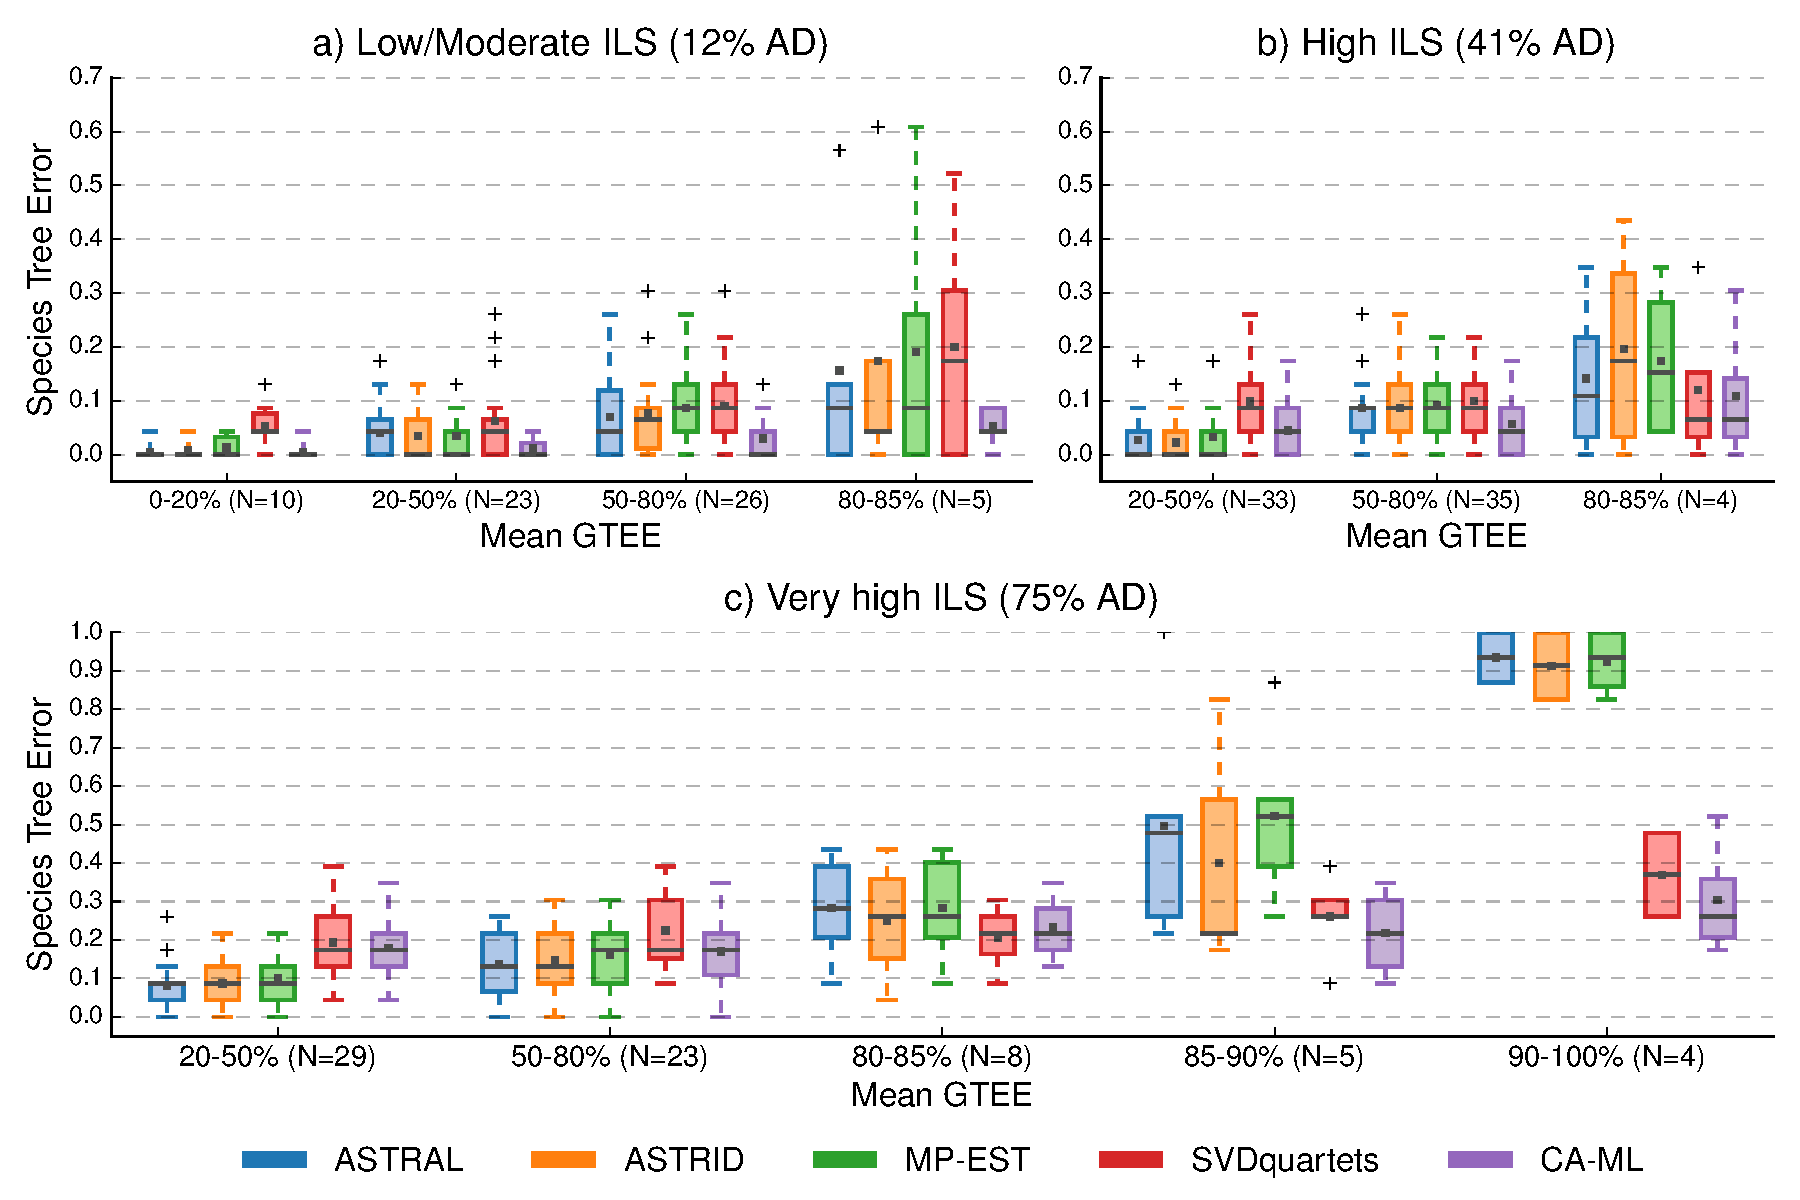
\includegraphics[width=1.0\textwidth]{figures/gene-filtering-fig1.pdf}
\caption{{\bf Impact of GTEE.} The impact of GTEE and ILS on species tree error (RF error rate) is shown for methods: ASTRAL-II (blue), ASTRID (orange), MP-EST (green), SVDquartets (red), and CA-ML using RAxML (purple). 
Subplots a, b, and c show three levels of increasing ILS. 
The mean GTEE range and the number of replicates ($N$) for that model condition are given on the $x$-axis. 
Means and medians are denoted by the gray dot and bar, respectively. Box plots are defined by quartiles, e.g., boxes extend from the first to the third quartiles. 
Greater levels of ILS and/or GTEE increased species tree error rates for all methods, and the relative performance of methods depended on both ILS and GTEE. 
Under low to moderate ILS, CA-ML tended to have better accuracy than the coalescent methods. 
Under higher levels of ILS, summary methods were typically more accurate than CA-ML and SVDquartets except for conditions with high GTEE.}
\label{fig:include-1}
\end{figure}

%\clearpage

\begin{figure}[!h]
\centering
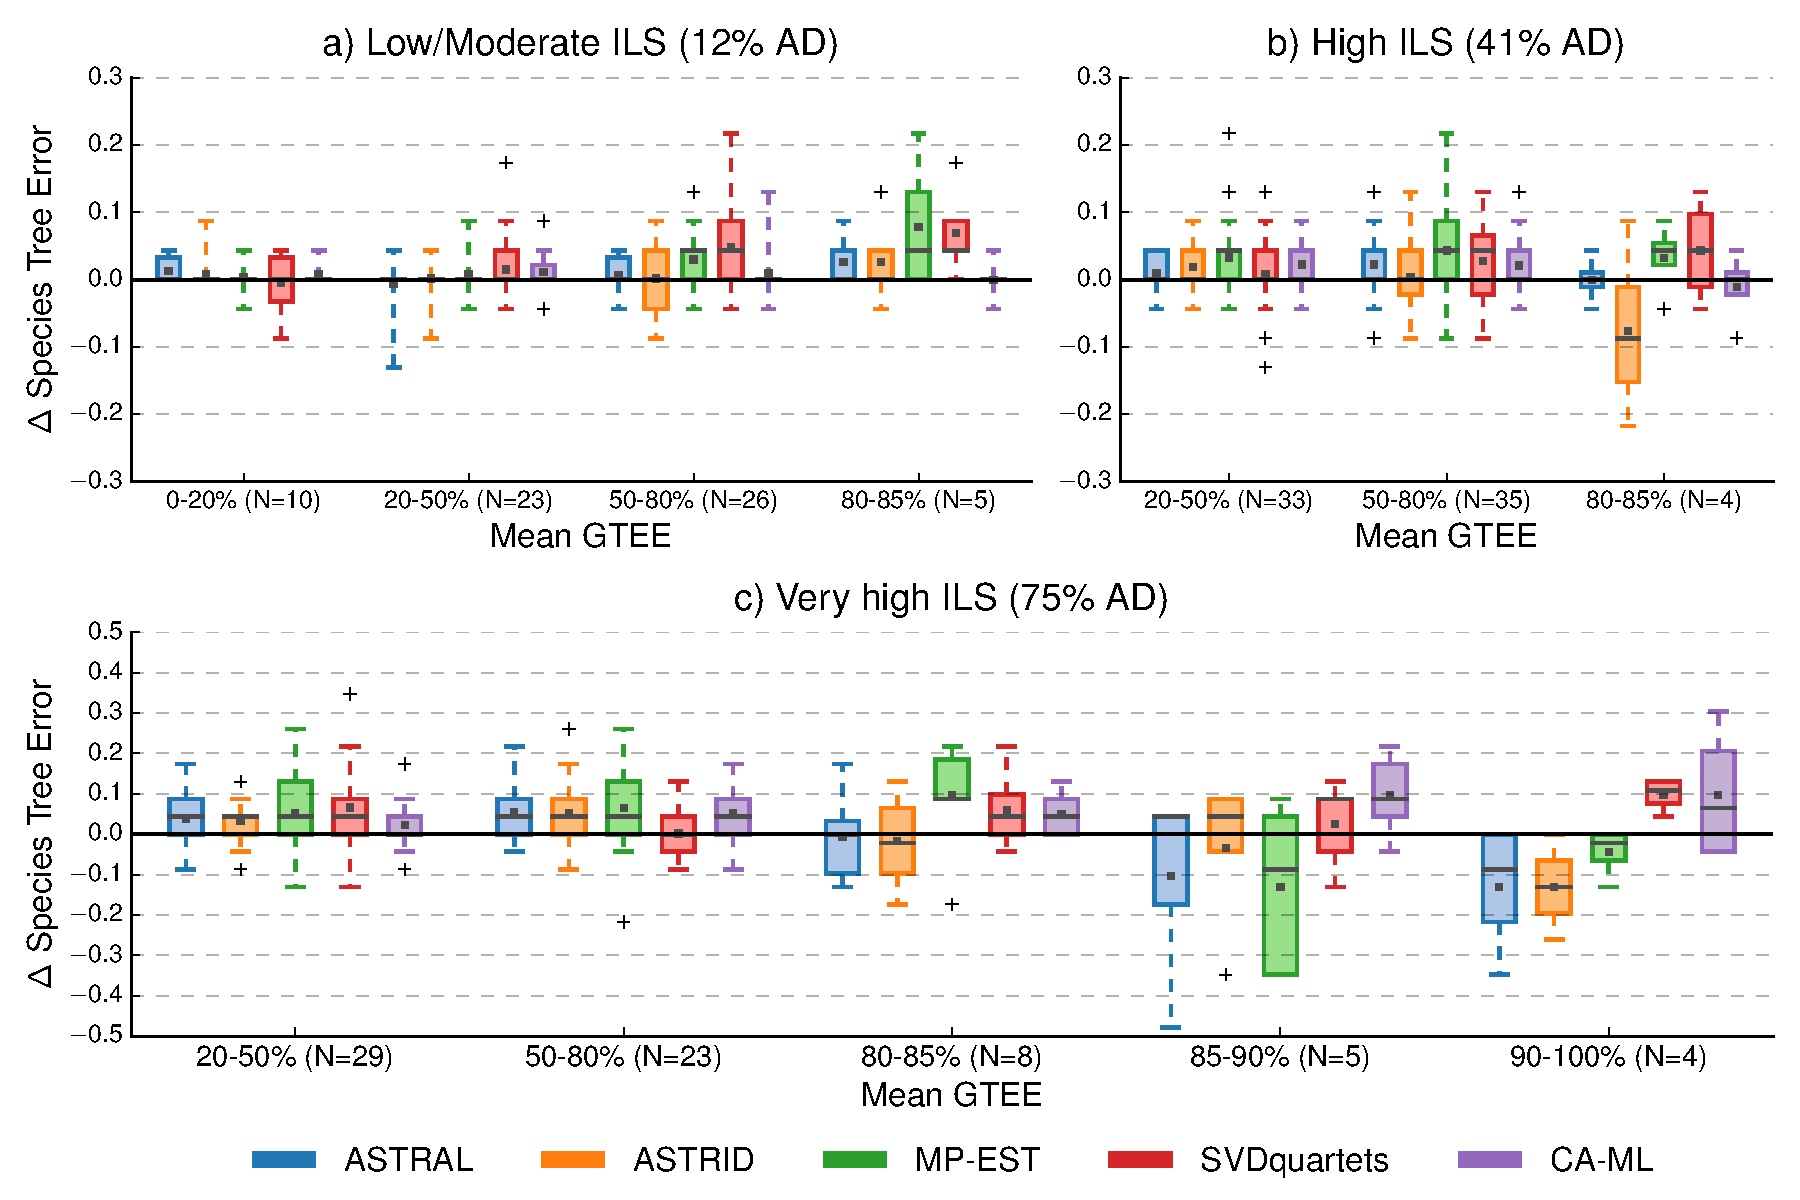
\includegraphics[width=1.0\textwidth]{figures/gene-filtering-fig2.pdf}
\caption{{\bf Impact of missing data.} Differences in species tree error between datasets with no missing data and datasets with approximately 30\% missing data are shown for five methods: ASTRAL-II (blue), ASTRID (orange), MP-EST (green), SVDquartets (red), and CA-ML using RAxML (purple). 
Positive values indicate increases in error, whereas negative values indicate reductions in error. 
Subplots a, b, and c show three levels of increasing ILS. 
The mean GTEE range and the number of replicates ($N$) for that model condition are given on the $x$-axis. 
Means and medians are denoted by the gray dot and bar, respectively. 
Box plots are defined by quartiles, e.g., boxes extend from the first to the third quartiles.}
\label{fig:include-2}
\end{figure}

%\clearpage

\begin{figure}[!h]
\centering
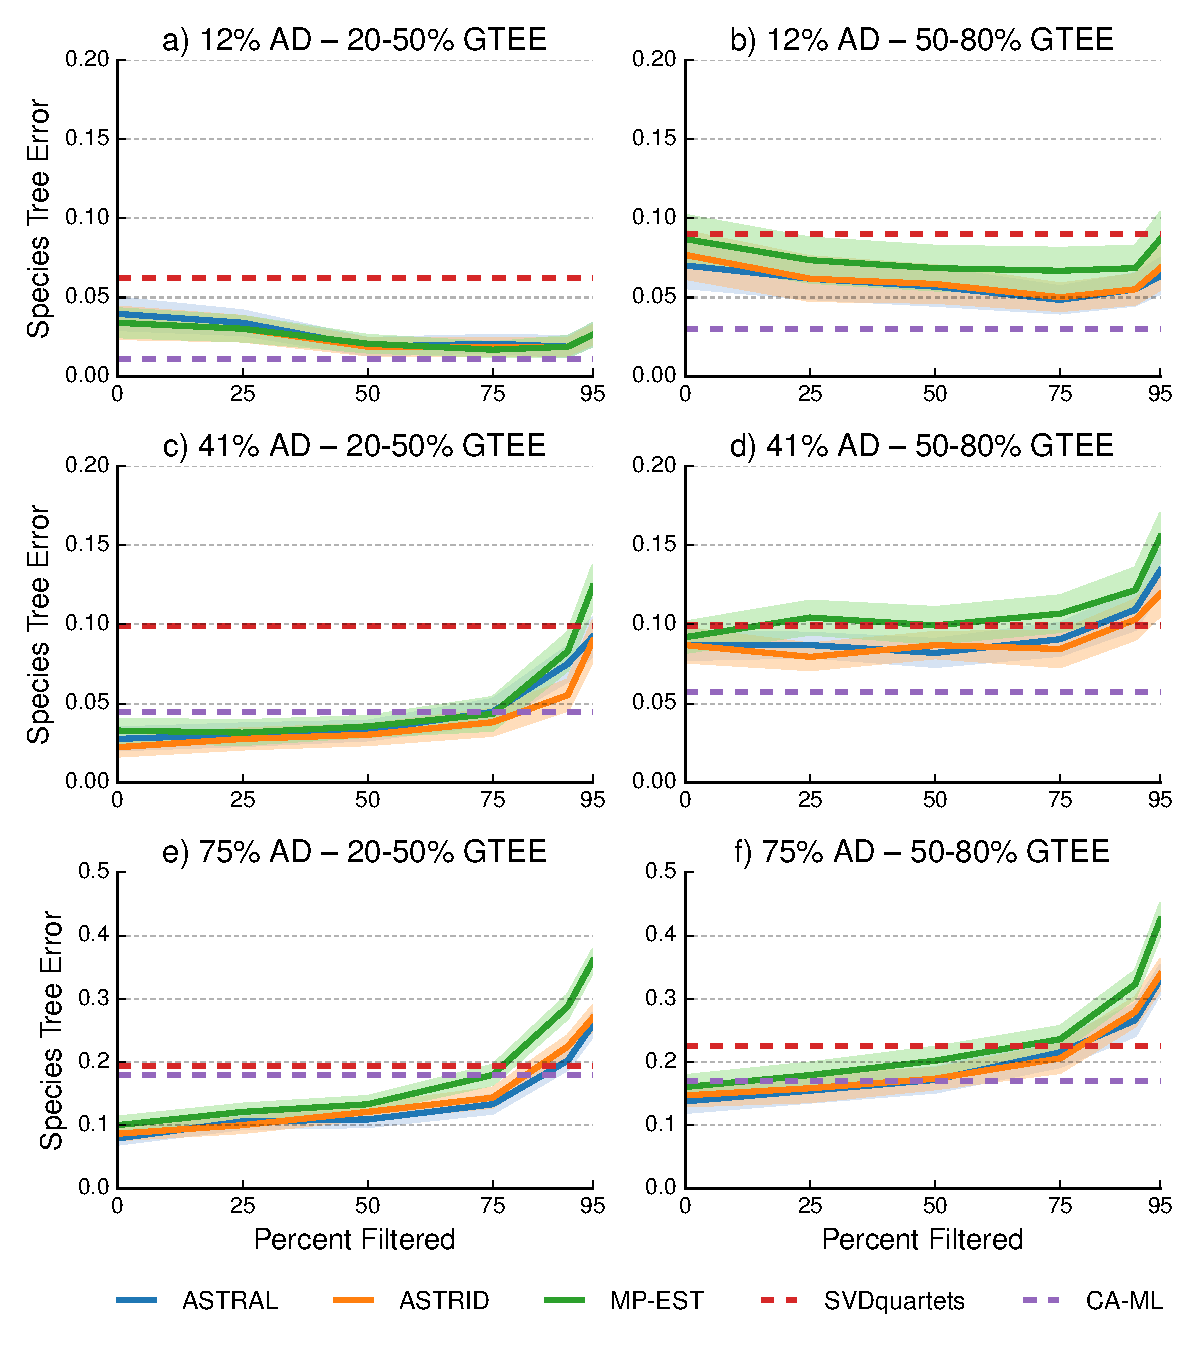
\includegraphics[width=0.80\textwidth]{figures/gene-filtering-fig3.pdf}
\caption{{\bf Impact of filtering based on GTEE.} The impact of filtering genes based on GTEE on species tree error (RF error rate) is shown for three summary methods: ASTRAL-II (solid blue), ASTRID (solid orange), and MP-EST (solid green). 
Genes were filtered by removing the top 25\%, 50\%, 75\%, 90\%, and 95\% of genes with the highest GTEE. 
SVDquartets (dashed red) and unpartitioned concatenation analysis CA-ML using RAxML (dashed purple), are shown without filtering. 
Lines indicate the mean across all replicates, and filled regions indicate the standard error. 
Rows show three levels of ILS, and  columns show two levels of GTEE. 
When ILS was sufficiently low, gene filtering (up to 75\% of genes) increased the accuracy of gene tree summary methods (a-b). When ILS was high to very high, gene filtering had little impact on the accuracy of summary methods or else reduced summary method accuracy (d-f).}
\label{fig:include-3}
\end{figure}

%\clearpage

\begin{figure}[!h]
\centering
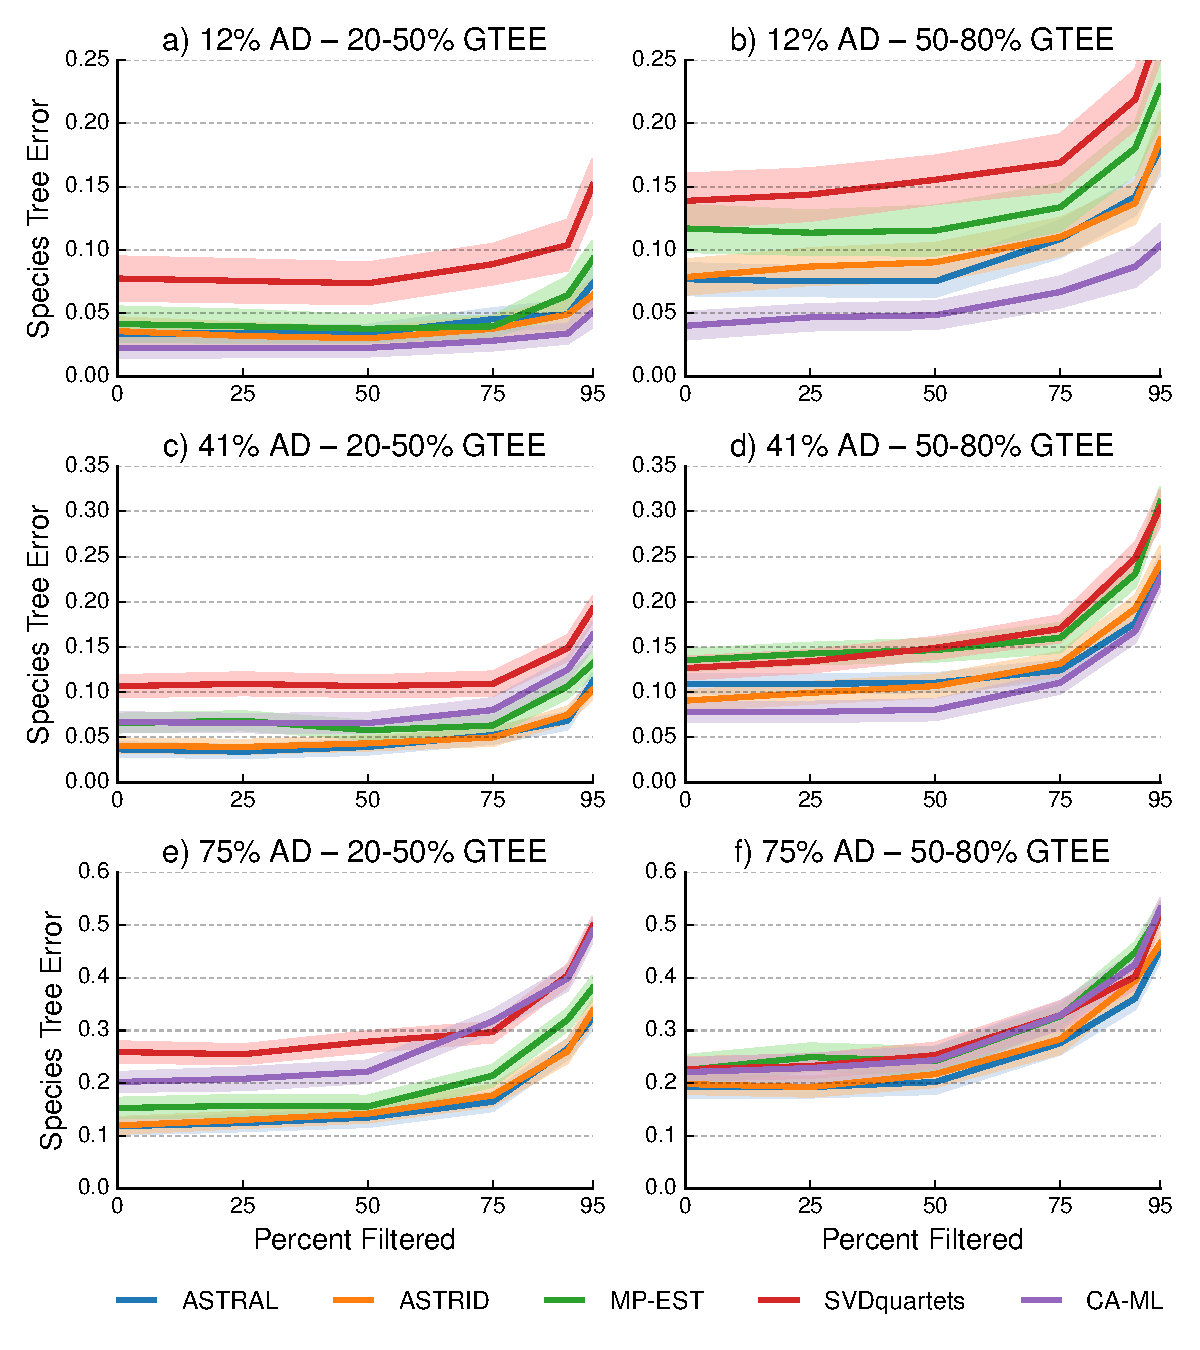
\includegraphics[width=0.80\textwidth]{figures/gene-filtering-fig4.pdf}
\caption{{\bf Impact of filtering based on missing data.} The impact of filtering genes by missing data on species tree error (RF error rate) is shown for five methods: ASTRAL-II (blue), ASTRID (orange), MP-EST (green), SVDquartets (red), and CA-ML using RAxML (purple). 
Genes were filtered by removing the top 25\%, 50\%, 75\%, 90\%, and 95\% of genes with the highest fractions of missing data; this resulted in removing genes missing at least 50\%, 25\%, 10\%, 5\%, and 1\% of species. 
Lines indicate the mean across all replicates, and filled regions indicate the standard error. 
Rows show three levels of increasing ILS, and columns show two levels of GTEE. 
Gene filtering based on missing data was at best neutral but often reduced the accuracy of methods.}
\label{fig:include-4}
\end{figure}

\begin{landscape}
\glsreset{parsimony-informative}
\section{Tables}
\label{sec:include-tables}
This section contains two tables: one presented in Section~\ref{sec:include-intro} Introduction  and one presented in Section~\ref{sec:include-results} Results.

\vspace{12pt}

\begin{table}[!h]
\caption{{\bf Empirical statistics for biological datasets.} 
Means and standard deviations across all genes are reported for the following quantities: MSA length, number of \textit{\gls{parsimony-informative}} sites (sites with at least two character states appearing at least twice), mean bootstrap support, and normalized RF distance between a gene tree and the species tree estimated via CA-ML.
Empirical statistics were computed using the MSAs, bootstrap gene trees, and CA-ML trees provided by these studies. 
In particular, we used the bootstrap gene trees (for each gene) to build a greedy consensus tree and a \textit{\gls{SMC}} tree (all bipartitions in the SMC tree are induced by greater than 50\% of the bootstrapped trees).
The greedy consensus tree was used to compute mean bootstrap support by averaging the bootstrap support values across all branches. 
The SMC tree was used to compute the distance between a gene tree and the species tree computed using CA-ML. 
The distance between the SMC tree and the estimated species tree is separated into False Positive (FP) rate and False Negative (FN) rate. 
FN rate is the fraction of branches in the estimated species tree that are missing from the SMC tree; FP rate is the fraction of branches in the SMC tree that are missing from the CA-ML tree. 
Note that Streicher {\em et al.} \cite{streicher2016how} provided concatenated alignments but not alignments for the individual genes in their Dryad repository, so the mean gene length and the mean number of parsimony informative sites per gene could not be computed.
}\label{tab:include-1}
\centering
\small
\begin{tabular}{l cccc cc cc}
\toprule
& Dataset & Number & Number & Gene & Number of & Mean bootstrap & \multicolumn{2}{c}{SMC versus CA-ML}\\[0.5ex]
Study & type & of species & of gene & length & informative sites & support & FP & FN \\
\midrule
Blom {\em et al.} \cite{blom2017accounting} & exon & 29 & 1361 & 384 $\pm$ 251 & 12 $\pm$ 10 & $0.28 \pm 0.11$ & $0.45 \pm 0.26$ & $0.87 \pm 0.09$ \\[0.5ex]
Hosner {\em et al.} \cite{hosner2016empirical} & \gls{UCE} & 91 & 4817 & 462 $\pm$ 369 & 37 $\pm$ 42 & $0.28 \pm 0.12$ &  $0.37 \pm 0.25$ & $0.83 \pm 0.17$ \\[0.5ex]
Jarvis {\em et al.} \cite{jarvis2014whole} & exon & 48 & 8251 & 1612 $\pm$ 1308 & 453 $\pm$ 418&  $0.26 \pm 0.07$ & $0.22 \pm 0.25$ & $0.85 \pm 0.08$ \\[0.5ex]
Jarvis {\em et al.} \cite{jarvis2014whole} & \gls{intron} & 48 & 2516 & 7654 $\pm$ 8539 & 4315 $\pm$ 4654 & $0.47 \pm 0.12$ & $0.20 \pm 0.13$ & $0.68 \pm 0.09$ \\[0.5ex]
Jarvis {\em et al.} \cite{jarvis2014whole} & UCE & 48 & 3679 & 2509 $\pm$ 164 & 1062 $\pm$ 278 & $0.40 \pm 0.05$ & $0.11 \pm 0.11$ & $0.71 \pm 0.03$ \\[0.5ex]
Streicher {\em et al.} \cite{streicher2016how} & UCE & 29 & 4784 & NA & NA & $0.39 \pm 0.09$ & $0.36 \pm 0.26$ & $0.78 \pm 0.12$ \\[0.5ex]
\bottomrule
\end{tabular}
\end{table}
\fillandplacepagenumber
\end{landscape}

\begin{landscape}
\begin{table}[!h]
\caption{{\bf Proportions of replicates for which filtering based on GTEE increased or decreased the accuracy of ASTRAL-II.} The proportion of replicates for which filtering based on GTEE increased and decreased the accuracy of ASTRAL-II is given on the left and right of the forward slash, respectively. The larger of these two values is in bold. If these two fractions do not sum to one, then the remainder is the proportion of replicates for which filtering did not impact accuracy. The number of replicates as well as the mean ($\pm$ standard deviation) of parsimony informative sites is given for each model condition, specified by the level of ILS and the range of mean GTEE.
}\label{tab:include-2}
\centering
\footnotesize
\begin{tabular}{rc cccccc}
\toprule
Mean & Number of & Number of & \multicolumn{5}{c}{Proportion of replicates affected by filtering (increased / decreased accuracy)} \\[0.5ex]
GTEE & replicates & informative sites & \multicolumn{5}{c}{when the following percentages of genes were removed}\\\cmidrule{4-8}
& & & 25\% & 50\% & 75\% & 90\% & 95\% \\
\midrule
\multicolumn{8}{l}{\em Low/Moderate ILS (12\% AD)}\\[0.5ex]
0-20\%  & 10 & 596 $\pm$ 224  & 0.00 / 0.00 & 0.00 / 0.00 & 0.00 / {\bf 0.10} & 0.00 / 0.00 & 0.00 / {\bf 0.20} \\[0.5ex]
20-50\%  & 23 & 464 $\pm$ 276  & {\bf 0.09} / 0.04 & {\bf 0.26} / 0.00 & {\bf 0.35} / 0.09 & {\bf 0.30} / 0.04 & {\bf 0.26} / 0.13 \\[0.5ex]
50-80\%  & 26 & 63 $\pm$ 14  & {\bf 0.23} / 0.04 & {\bf 0.23} / 0.04 & {\bf 0.31} / 0.12 & {\bf 0.35} / 0.23 & {\bf 0.35} / 0.31 \\[0.5ex]
80-85\%  & 5 & 40 $\pm$ 28  & 0.40 / {\bf 0.60} & 0.40 / 0.40 & 0.40 / {\bf 0.60} & 0.20 / {\bf 0.60} & 0.20 / {\bf 0.80} \\[0.5ex]
85-100\%  & 2 & 5 $\pm$ 3  & {\bf 0.50} / 0.00 & {\bf 1.00} / 0.00 & {\bf 1.00} / 0.00 & {\bf 1.00} / 0.00 & {\bf 1.00} / 0.00 \\[2ex]
\multicolumn{8}{l}{\em High ILS (41\% AD)}\\[0.5ex]
0-20\%  & 2 & 487 $\pm$ 9  & 0.00 / {\bf 0.50} & 0.00 / {\bf 0.50} & 0.00 / {\bf 1.00} & 0.00 / 0.00 & 0.00 / {\bf 0.50} \\[0.5ex]
20-50\%  & 33 & 349 $\pm$ 208  & 0.03 / {\bf 0.09} & 0.15 / {\bf 0.27} & 0.15 / {\bf 0.33} & 0.03 / {\bf 0.55} & 0.03 / {\bf 0.70} \\[0.5ex]
50-80\%  & 35 & 42 $\pm$ 17  & 0.11 / {\bf 0.17} & {\bf 0.26} / 0.17 & 0.26 / {\bf 0.34} & 0.14 / {\bf 0.49} & 0.17 / {\bf 0.60} \\[0.5ex]
80-85\%  & 4 & 22 $\pm$ 10  & {\bf 0.75} / 0.00 & {\bf 0.50} / 0.00 & {\bf 0.25} / 0.00 & 0.25 / 0.25 & 0.25 / {\bf 0.50} \\[0.5ex]
85-100\%  & 1 & 6 $\pm$ 0  & 0.00 / 0.00 & {\bf 1.00} / 0.00 & {\bf 1.00} / 0.00 & {\bf 1.00} / 0.00 & {\bf 1.00} / 0.00 \\[2ex]
\multicolumn{8}{l}{\em Very high ILS (75\% AD)}\\[0.5ex]
0-20\%  & 0 & NA & NA & NA & NA & NA & NA \\[0.5ex]
20-50\%  & 29 & 213 $\pm$ 123  & 0.07 / {\bf 0.45} & 0.07 / {\bf 0.59} & 0.14 / {\bf 0.59} & 0.00 / {\bf 0.93} & 0.00 / {\bf 1.00} \\[0.5ex]
50-80\%  & 23 & 30 $\pm$ 9  & 0.22 / {\bf 0.35} & 0.17 / {\bf 0.61} & 0.09 / {\bf 0.70} & 0.04 / {\bf 0.87} & 0.00 / {\bf 1.00} \\[0.5ex]
80-85\%  & 8 & 17 $\pm$ 10  & {\bf 0.75} / 0.00 & {\bf 0.62} / 0.25 & {\bf 0.62} / 0.25 & {\bf 0.50} / 0.38 & 0.00 / {\bf 0.75} \\[0.5ex]
85-100\%  & 9 & 6 $\pm$ 6  & {\bf 0.56} / 0.00 & {\bf 0.67} / 0.00 & {\bf 0.78} / 0.00 & {\bf 0.78} / 0.11 & {\bf 0.78} / 0.22 \\[0.5ex]
\bottomrule
\end{tabular}
\end{table}
\fillandplacepagenumber
\end{landscape}